%\renewcommand{\theequation}{\theenumi}
\begin{enumerate}[label=\thesubsection.\arabic*.,ref=\thesubsection.\theenumi]
%\numberwithin{equation}{enumi}
\item The direction vector of $AB$ is defined as
		\begin{align}
			\vec{B}-
			\vec{A}
		\end{align}
Find the direction vectors of $AB, BC$ and $CA$.
\\
\solution 
\begin{enumerate} 
\item  The Direction vector of $AB$ is 
	\begin{align}  \vec{B} - \vec{A} 
		=\myvec{ -4\\ 6 } - \myvec{ 1\\ -1 }
 = \myvec{ -4 - 1\\ 6 - (-1) } = \myvec{ -5\\ 7 }
		\label{eq:app-geo-dir-vec-ab}
 \end{align}
\item The Direction vector of $BC$ is
	\begin{align} \vec{C} - \vec{B}=\myvec{ -3\\ -5} - \myvec{ -4\\ 6 }
 = \myvec{ -3 - (-4)\\ -5 - 6 } = \myvec{1\\ -11 }
		\label{eq:app-geo-dir-vec-bc}
  \end{align}
  \item  The Direction vector of $CA$  is
	  \begin{align}  \vec{A} - \vec{C} =\myvec{ 1\\ -1 }-\myvec{ -3\\ -5}
 = \myvec{ 1 - (-3)\\ -1 - (-5) } = \myvec{ 4\\ 4 }
		\label{eq:app-geo-dir-vec-ca}
  \end{align}
 \end{enumerate}
%	\solution 
\begin{enumerate} 
\item  The Direction vector of $AB$ is 
	\begin{align}  \vec{B} - \vec{A} 
		=\myvec{ -4\\ 6 } - \myvec{ 1\\ -1 }
 = \myvec{ -4 - 1\\ 6 - (-1) } = \myvec{ -5\\ 7 }
		\label{eq:geo-dir-vec-ab}
 \end{align}
\item The Direction vector of $BC$ is
	\begin{align} \vec{C} - \vec{B}=\myvec{ -3\\ -5} - \myvec{ -4\\ 6 }
 = \myvec{ -3 - (-4)\\ -5 - 6 } = \myvec{1\\ -11 }
		\label{eq:geo-dir-vec-bc}
  \end{align}
  \item  The Direction vector of $CA$  is
	  \begin{align}  \vec{A} - \vec{C} =\myvec{ 1\\ -1 }-\myvec{ -3\\ -5}
 = \myvec{ 1 - (-3)\\ -1 - (-5) } = \myvec{ 4\\ 4 }
		\label{eq:geo-dir-vec-ca}
  \end{align}
 \end{enumerate}


	\item The length of side $BC$ is 
		\label{prob:side-length}
		\begin{align}
			c = \norm{\vec{B}-\vec{A}} \triangleq \sqrt{\brak{\vec{B}-\vec{A}}^{\top}\brak{\vec{B}-\vec{A}}}
		\end{align}
		where
		\begin{align}
			\vec{A}^{\top}\triangleq\myvec{1 & -1}
		\end{align}
		Similarly, 
		\begin{align}
b = \norm{\vec{C}-\vec{B}},\,
a = \norm{\vec{A}-\vec{C}}
		\end{align}
		Find $a, b, c$.
\begin{enumerate}
	\item 
	From 	
		\eqref{eq:app-geo-dir-vec-ab},
\begin{align}
\vec{A}-\vec{B} &= \myvec{5\\-7}, \\
\implies 	c &= 	\norm{\vec{B}-\vec{A}} = \norm{\vec{A}-\vec{B}} 
	\\
	&= \sqrt{\myvec{5 & -7}\myvec{5\\-7}}
= \sqrt{\brak{5}^2 +\brak{7}^2}\\
	&=\sqrt{74}
		\label{eq:app-geo-norm-ab}
\end{align}
	\item Similarly, from 
		\eqref{eq:app-geo-dir-vec-bc},
\begin{align}
	a &= \norm{\vec{B}-\vec{C}} 
	= \sqrt{\myvec{-1 & 11}\myvec{-1\\11}}
\\
&= \sqrt{\brak{1}^2+\brak{11}^2}
	= \sqrt{122}
		\label{eq:app-geo-norm-bc}
\end{align}
and
		from 		\eqref{eq:app-geo-dir-vec-ca},
	\item 
		\begin{align}
			b &= \norm{\vec{A}-\vec{C}} = \sqrt{\myvec{4 & 4}\myvec{4\\4}}
\\
&= \sqrt{\brak{4}^2+\brak{4}^2}
	=\sqrt{32}
		\label{eq:app-geo-norm-ca}
\end{align}
\end{enumerate}
\begin{lstlisting}
	codes/msoft/sides.c
\end{lstlisting}
%  \\            
  %\begin{enumerate}
	\item 
	From 	
		\eqref{eq:geo-dir-vec-ab},
\begin{align}
\vec{A}-\vec{B} &= \myvec{5\\-7}, \\
\implies 	c &= 	\norm{\vec{B}-\vec{A}} = \norm{\vec{A}-\vec{B}} 
	\\
	&= \sqrt{\myvec{5 & -7}\myvec{5\\-7}}
= \sqrt{\brak{5}^2 +\brak{7}^2}\\
	&=\sqrt{74}
		\label{eq:geo-norm-ab}
\end{align}
	\item Similarly, from 
		\eqref{eq:geo-dir-vec-bc},
\begin{align}
	a &= \norm{\vec{B}-\vec{C}} 
	= \sqrt{\myvec{-1 & 11}\myvec{-1\\11}}
\\
&= \sqrt{\brak{1}^2+\brak{11}^2}
	= \sqrt{122}
		\label{eq:geo-norm-bc}
\end{align}
and
		from 		\eqref{eq:geo-dir-vec-ca},
	\item 
		\begin{align}
			b &= \norm{\vec{A}-\vec{C}} = \sqrt{\myvec{4 & 4}\myvec{4\\4}}
\\
&= \sqrt{\brak{4}^2+\brak{4}^2}
	=\sqrt{32}
		\label{eq:geo-norm-ca}
\end{align}
\end{enumerate}

\item   Points $\vec{A}, \vec{B}, \vec{C}$ are defined to be collinear if 
		\begin{align}
			\label{eq:app-app-line-rank}
			\rank{\myvec{1 & 1 & 1 \\ \vec{A}& \vec{B}&\vec{C}}} = 2
		\end{align}
Are the given points in
			\eqref{eq:app-tri-pts}
collinear?
\\
\solution 
From 
			\eqref{eq:app-tri-pts},
\begin{align}
    \label{eq:app-1.1.3,2}
\myvec{
    1 & 1 & 1\\
    \vec{A} & \vec{B} & \vec{C} \\
    } 
    =
    %\label{eq:app-matthrowoperations}
    \myvec{
    1 & 1 & 1
    \\
    1 & -4 & -3
    \\
    -1 & 6 & -5
    }
     \xleftrightarrow[]{R_3 \leftarrow R_3+R_2}
    \myvec{
    1 & 1 & 1
    \\
    1 & -4 & -3
    \\
    0 & 2 & -8 
    }
    \\
     \xleftrightarrow[]{R_2\leftarrow R_1-R_2}
    \myvec{
    1 & 1 & 1
    \\
    0 & 5 & 4
    \\
    0 & 2 & -8 
    }
     \xleftrightarrow[]{R_3\leftarrow R_3-\frac{2}{5}R_2}
    \myvec{
    1 & 1 & 1
    \\
    0 & 5 & 4
    \\
    0 & 0 & \frac{-48}{5}
    }
\end{align}
There are no zero rows. So,
\begin{align}
    \text{rank}\myvec{
    1 & 1 & 1\\
    \vec{A} & \vec{B} & \vec{C} \\
    } &= 3 
\end{align}  
Hence,  the points $\vec{A},\vec{B},\vec{C}$ are not collinear. 
This is visible in 
\figref{fig1:Triangle}.
\begin{figure}[H]
\centering
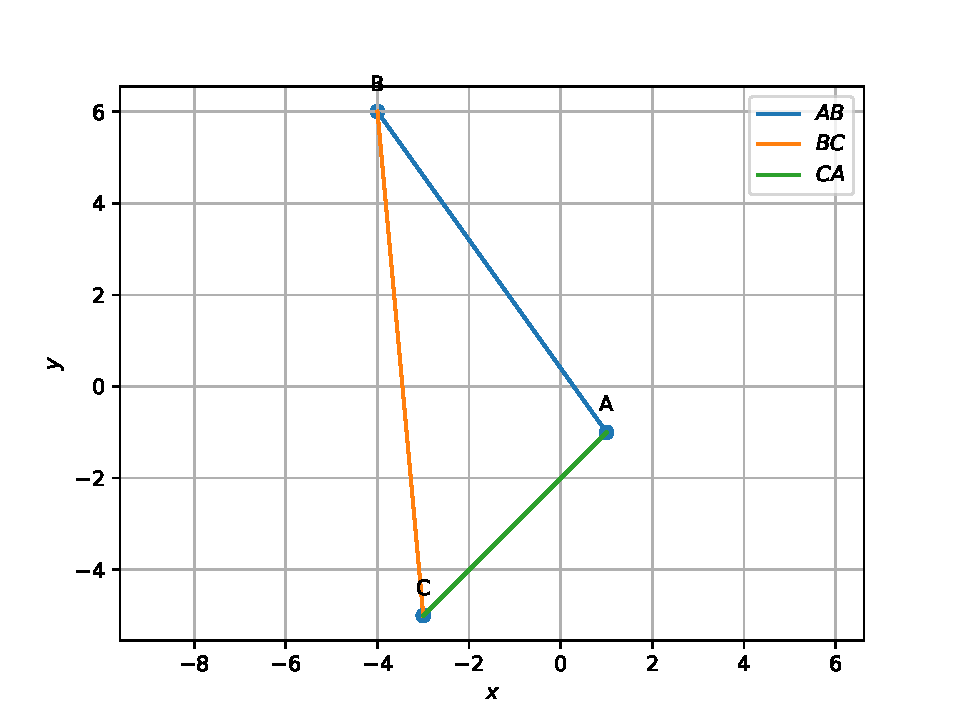
\includegraphics[width=0.75\columnwidth]{figs/triangle/vector.pdf}
\caption{$\triangle ABC$}
\label{fig1:Triangle}
\end{figure}
% \\		\solution 
From 
			\eqref{eq:tri-pts},
\begin{align}
    \label{eq:1.1.3,2}
\myvec{
    1 & 1 & 1\\
    \vec{A} & \vec{B} & \vec{C} \\
    } 
    =
    %\label{eq:matthrowoperations}
    \myvec{
    1 & 1 & 1
    \\
    1 & -4 & -3
    \\
    -1 & 6 & -5
    }
     \xleftrightarrow[]{R_3 \leftarrow R_3+R_2}
    \myvec{
    1 & 1 & 1
    \\
    1 & -4 & -3
    \\
    0 & 2 & -8 
    }
    \\
     \xleftrightarrow[]{R_2\leftarrow R_1-R_2}
    \myvec{
    1 & 1 & 1
    \\
    0 & 5 & 4
    \\
    0 & 2 & -8 
    }
     \xleftrightarrow[]{R_3\leftarrow R_3-\frac{2}{5}R_2}
    \myvec{
    1 & 1 & 1
    \\
    0 & 5 & 4
    \\
    0 & 0 & \frac{-48}{5}
    }
\end{align}
There are no zero rows. So,
\begin{align}
    \text{rank}\myvec{
    1 & 1 & 1\\
    \vec{A} & \vec{B} & \vec{C} \\
    } &= 3 
\end{align}  
Hence,  the points $\vec{A},\vec{B},\vec{C}$ are not collinear. 
This is visible in 
\figref{fig1:Triangle}.
\begin{figure}[H]
\centering
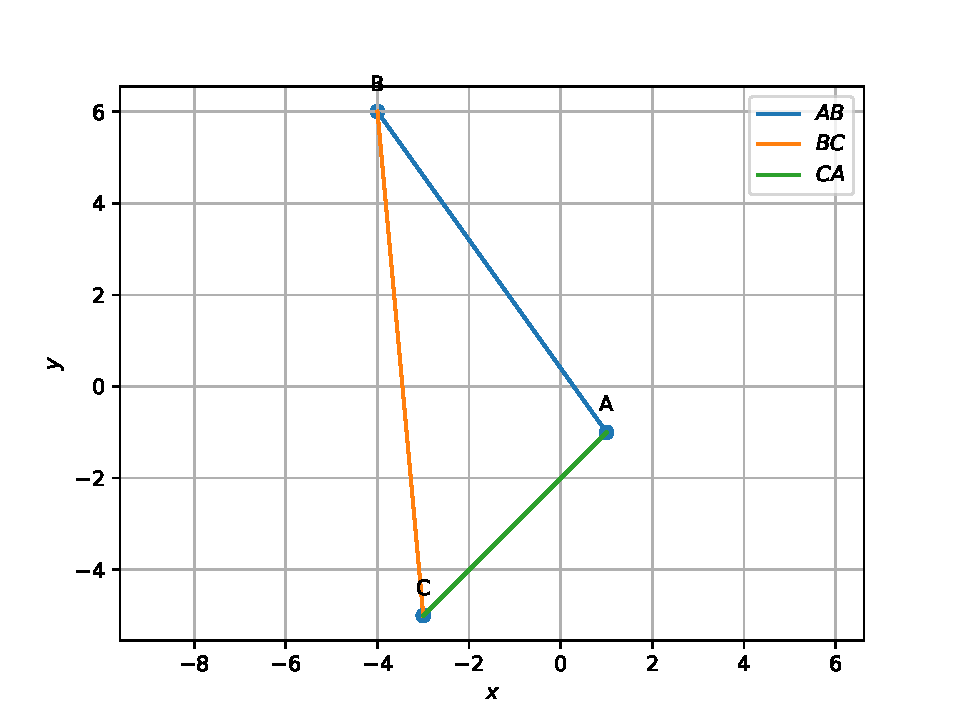
\includegraphics[width=0.75\columnwidth]{figs/triangle/vector.pdf}
\caption{$\triangle ABC$}
\label{fig1:Triangle}
\end{figure}

\item The parameteric form of the equation  of $AB$ is 
		\begin{align}
			\label{eq:app-geo-param}
			\vec{x}=\vec{A}+k\vec{m} \quad k \ne 0,
		\end{align}
		where
		\begin{align}
\vec{m}=\vec{B}-\vec{A}
		\end{align}
is the direction vector of $AB$.
Find the parameteric equations of $AB, BC$ and $CA$.
\\
\solution
From 
			\eqref{eq:app-geo-param} and
		\eqref{eq:app-geo-dir-vec-ab},
the parametric equation for $AB$ is given by
\begin{align}
AB: \vec{x} = &\myvec{1\\-1} + k \myvec{-5\\7}
\end{align}
Similarly, from 
		\eqref{eq:app-geo-dir-vec-bc} and
		\eqref{eq:app-geo-dir-vec-ca},
\begin{align}
BC: \vec{x} = &\myvec{-4\\6} + k \myvec{1\\-11}\\
CA: \vec{x} = &\myvec{-3\\-5} + k \myvec{4\\4}
\end{align}

%		\solution
From 
			\eqref{eq:geo-param} and
		\eqref{eq:geo-dir-vec-ab},
the parametric equation for $AB$ is given by
\begin{align}
AB: \vec{x} = &\myvec{1\\-1} + k \myvec{-5\\7}
\end{align}
Similarly, from 
		\eqref{eq:geo-dir-vec-bc} and
		\eqref{eq:geo-dir-vec-ca},
\begin{align}
BC: \vec{x} = &\myvec{-4\\6} + k \myvec{1\\-11}\\
CA: \vec{x} = &\myvec{-3\\-5} + k \myvec{4\\4}
\end{align}


\item The normal form of the equation of $AB$  is 
		\begin{align}
			\label{eq:app-geo-normal}
			\vec{n}^{\top}\brak{	\vec{x}-\vec{A}} = 0
		\end{align}
		where 
		\begin{align}
			\vec{n}^{\top}\vec{m}&=\vec{n}^{\top}\brak{\vec{B}-\vec{A}} = 0
			\\
			\text{or, } \vec{n}&=\myvec{0 & 1 \\ -1 & 0} \vec{m}
			\label{eq:app-geo-norm-vec}
		\end{align}
Find the normal form of the equations of $AB, BC$ and $CA$.
\\
\solution
\begin{enumerate}
	\item
From
		\eqref{eq:app-geo-dir-vec-bc}, 
the direction vector of side $\vec{BC}$ is
\begin{align}
\vec{m}
	&=\myvec{1\\-11}
	\\
\implies \vec{n} &= \myvec{0 & 1\\
  -1 & 0}\myvec{1\\-11}
 = \myvec{-11\\-1}
		\label{eq:app-geo-norm-vec-bc}
\end{align}
from 
			\eqref{eq:app-geo-norm-vec}.
Hence, from 
			\eqref{eq:app-geo-normal},
the normal equation of side $BC$ is 
\begin{align}
	\vec{n}^{\top}\brak{	\vec{x}-\vec{B}} &= 0
			\\
\implies    \myvec{-11 & -1}\vec{x}&=\myvec{-11 & -1}\myvec{-4\\6}\\
    \implies
BC: \quad    \myvec{11 & 1}\vec{x}&=-38
\end{align}
\item Similarly, for $AB$,
from 
		\eqref{eq:app-geo-dir-vec-ab}, 
\begin{align}
	\vec{m} &= \myvec{-5\\7}
	\\
\implies        \vec{n} 
                &= \myvec{0&1\\-1&0}\myvec{-5\\7}
                = \myvec{7\\5}
		\label{eq:app-geo-norm-vec-ab}
\end{align}
and 
\begin{align}
	\vec{n}^{\top}\brak{	\vec{x}-\vec{A}} &= 0
	\\
	\implies
                AB: \quad  \vec{n}^{\top}\vec{x} &= \myvec{7&5}\myvec{1\\-1}\\    
       \implies\myvec{7&5}\vec{x} &= 2
\end{align}
\item For 
$CA$, 
from 
		\eqref{eq:app-geo-dir-vec-ca}, 
\begin{align}
\vec{m} &= \myvec{1 \\ 1}
\\
		\label{eq:app-geo-norm-vec-ca}
\implies \vec{n} 
&= \myvec{0&1 \\ -1&0}\myvec{1 \\ 1}
= \myvec{1 \\ -1}\\
\\
\implies	\vec{n}^{\top}\brak{	\vec{x}-\vec{C}} &= 0
\\
\implies \myvec{1&-1}{\vec{x}} &= \myvec{1&-1}\myvec{-3 \\ -5} 
= 2 
\end{align}
\end{enumerate}

%\begin{enumerate}
	\item
From
		\eqref{eq:geo-dir-vec-bc}, 
the direction vector of side $\vec{BC}$ is
\begin{align}
\vec{m}
	&=\myvec{1\\-11}
	\\
\implies \vec{n} &= \myvec{0 & 1\\
  -1 & 0}\myvec{1\\-11}
 = \myvec{-11\\-1}
		\label{eq:geo-norm-vec-bc}
\end{align}
from 
			\eqref{eq:geo-norm-vec}.
Hence, from 
			\eqref{eq:geo-normal},
the normal equation of side $BC$ is 
\begin{align}
	\vec{n}^{\top}\brak{	\vec{x}-\vec{B}} &= 0
			\\
\implies    \myvec{-11 & -1}\vec{x}&=\myvec{-11 & -1}\myvec{-4\\6}\\
    \implies
BC: \quad    \myvec{11 & 1}\vec{x}&=-38
\end{align}
\item Similarly, for $AB$,
from 
		\eqref{eq:geo-dir-vec-ab}, 
\begin{align}
	\vec{m} &= \myvec{-5\\7}
	\\
\implies        \vec{n} 
                &= \myvec{0&1\\-1&0}\myvec{-5\\7}
                = \myvec{7\\5}
		\label{eq:geo-norm-vec-ab}
\end{align}
and 
\begin{align}
	\vec{n}^{\top}\brak{	\vec{x}-\vec{A}} &= 0
	\\
	\implies
                AB: \quad  \vec{n}^{\top}\vec{x} &= \myvec{7&5}\myvec{1\\-1}\\    
       \implies\myvec{7&5}\vec{x} &= 2
\end{align}
\item For 
$CA$, 
from 
		\eqref{eq:geo-dir-vec-ca}, 
\begin{align}
\vec{m} &= \myvec{1 \\ 1}
\\
		\label{eq:geo-norm-vec-ca}
\implies \vec{n} 
&= \myvec{0&1 \\ -1&0}\myvec{1 \\ 1}
= \myvec{1 \\ -1}\\
\\
\implies	\vec{n}^{\top}\brak{	\vec{x}-\vec{C}} &= 0
\\
\implies \myvec{1&-1}{\vec{x}} &= \myvec{1&-1}\myvec{-3 \\ -5} 
= 2 
\end{align}
\end{enumerate}


\item The area of $\triangle ABC$ is defined as
		\begin{align}
			\label{eq:app-tri-area-cross}
			\frac{1}{2}\norm{{\brak{\vec{A}-\vec{B}}\times \brak{\vec{A}-\vec{C}}}}
		\end{align}
		where
		\begin{align}
			\vec{A}\times\vec{B} \triangleq \mydet{1 & -4 \\-1 & 6}
		\end{align}
		Find the area of $\triangle ABC$.\\
\solution
From
		\eqref{eq:app-geo-dir-vec-ab}
		and
		\eqref{eq:app-geo-dir-vec-ca},
\begin{align}
	\vec{A}-\vec{B}=\myvec{5\\-7},
	\vec{A}-\vec{C}&=\myvec{4\\4}\\
\implies (\vec{A}-\vec{B})\times(\vec{A}-\vec{C}) &=\mydet{5 & 4\\-7 & 4}\\
&=5\times 4-4\times (-7)\\&=48\\
\implies\frac{1}{2}\norm{(\vec{A}-\vec{B})\times(\vec{A}-\vec{C})}&=\frac{48}{2}=24
\end{align}
which is the desired area.

%  		\solution
From
		\eqref{eq:geo-dir-vec-ab}
		and
		\eqref{eq:geo-dir-vec-ca},
\begin{align}
	\vec{A}-\vec{B}=\myvec{5\\-7},
	\vec{A}-\vec{C}&=\myvec{4\\4}\\
\implies (\vec{A}-\vec{B})\times(\vec{A}-\vec{C}) &=\mydet{5 & 4\\-7 & 4}\\
&=5\times 4-4\times (-7)\\&=48\\
\implies\frac{1}{2}\norm{(\vec{A}-\vec{B})\times(\vec{A}-\vec{C})}&=\frac{48}{2}=24
\end{align}
which is the desired area.


	\item Find the angles $A, B, C$ if 
%    \label{prop:angle2d}
  \begin{align}
    \label{eq:app-angle2d}
			\cos A \triangleq 
\frac{\brak{\vec{B}-\vec{A}}^{\top}{\vec{C}-\vec{A}}}{\norm{\vec{B}-\vec{A}}\norm{\vec{C}-\vec{A}}}
  \end{align}\\
  \solution
\begin{enumerate}
	\item From 
		\eqref{eq:app-geo-dir-vec-ab},
		\eqref{eq:app-geo-dir-vec-ca},
		\eqref{eq:app-geo-norm-ab}
		and
		\eqref{eq:app-geo-norm-ca}
\begin{align}
	(\vec{B}-\vec{A})^{\top}(\vec{C}-\vec{A})&=\myvec{-5&7}\myvec{-4\\-4}\\
	&=-8
	\\
	\implies
	\cos{A}&= \frac{-8}{\sqrt{74} \sqrt{32}}
	= \frac{-1}{\sqrt{37}}\\
	\implies A&=\cos^{-1}{\frac{-1}{\sqrt{37}}}
\end{align}
	\item From 
		\eqref{eq:app-geo-dir-vec-ab},
		\eqref{eq:app-geo-dir-vec-bc},
		\eqref{eq:app-geo-norm-ab}
		and
		\eqref{eq:app-geo-norm-bc}
\begin{align}
	(\vec{C}-\vec{B})^{\top}(\vec{A}-\vec{B})&=\myvec{1&-11}\myvec{5\\-7}\\
	&= 82
	\\
	\implies
	\cos{B}&= \frac{82}{\sqrt{74} \sqrt{122}}
	= \frac{41}{\sqrt{2257}}\\
	\implies B&=\cos^{-1}{\frac{41}{\sqrt{2257}}}
\end{align}
	\item From 
		\eqref{eq:app-geo-dir-vec-bc},
		\eqref{eq:app-geo-dir-vec-ca},
		\eqref{eq:app-geo-norm-bc}
		and
		\eqref{eq:app-geo-norm-ca}
\begin{align}
	(\vec{A}-\vec{C})^{\top}(\vec{B}-\vec{C})&=\myvec{4&4}\myvec{-1\\11}\\
	&=40
	\\
\implies	\cos{C}&= \frac{40}{\sqrt{32} \sqrt{122}}
	= \frac{5}{\sqrt{61}}\\
	\implies C&=\cos^{-1}{\frac{5}{\sqrt{61}}}
\end{align}

\end{enumerate}
%  	\begin{enumerate}
	\item From 
		\eqref{eq:geo-dir-vec-ab},
		\eqref{eq:geo-dir-vec-ca},
		\eqref{eq:geo-norm-ab}
		and
		\eqref{eq:geo-norm-ca}
\begin{align}
	(\vec{B}-\vec{A})^{\top}(\vec{C}-\vec{A})&=\myvec{-5&7}\myvec{-4\\-4}\\
	&=-8
	\\
	\implies
	\cos{A}&= \frac{-8}{\sqrt{74} \sqrt{32}}
	= \frac{-1}{\sqrt{37}}\\
	\implies A&=\cos^{-1}{\frac{-1}{\sqrt{37}}}
\end{align}
	\item From 
		\eqref{eq:geo-dir-vec-ab},
		\eqref{eq:geo-dir-vec-bc},
		\eqref{eq:geo-norm-ab}
		and
		\eqref{eq:geo-norm-bc}
\begin{align}
	(\vec{C}-\vec{B})^{\top}(\vec{A}-\vec{B})&=\myvec{1&-11}\myvec{5\\-7}\\
	&= 82
	\\
	\implies
	\cos{B}&= \frac{82}{\sqrt{74} \sqrt{122}}
	= \frac{41}{\sqrt{2257}}\\
	\implies B&=\cos^{-1}{\frac{41}{\sqrt{2257}}}
\end{align}
	\item From 
		\eqref{eq:geo-dir-vec-bc},
		\eqref{eq:geo-dir-vec-ca},
		\eqref{eq:geo-norm-bc}
		and
		\eqref{eq:geo-norm-ca}
\begin{align}
	(\vec{A}-\vec{C})^{\top}(\vec{B}-\vec{C})&=\myvec{4&4}\myvec{-1\\11}\\
	&=40
	\\
\implies	\cos{C}&= \frac{40}{\sqrt{32} \sqrt{122}}
	= \frac{5}{\sqrt{61}}\\
	\implies C&=\cos^{-1}{\frac{5}{\sqrt{61}}}
\end{align}

\end{enumerate}

All codes for this section are available at
\begin{lstlisting}
	codes/triangle/sides.py
\end{lstlisting}
\end{enumerate}
